
\resetcounters

\markboth{Royer et al.}{The GIRAFFE Archive: 1D and 3D Spectra}


\title{The \ssindex{archives!individual!GIRAFFE}GIRAFFE Archive: 1D and \ssindex{spectroscopy!3D}3D Spectra}
\author{F.~Royer,$^1$ I.~J\'egouzo,$^1$ F.~Tajahmady,$^1$ J.~Normand,$^2$ and I.~Chilingarian$^3$
\affil{$^1$GEPI -- Observatoire de Paris}
\affil{$^2$VO Paris Data Center -- Observatoire de Paris}
\affil{$^3$Harvard-Smithsonian Center for Astrophysics}}

\aindex{Royer, F.}
\aindex{J\'egouzo, I.}
\aindex{Tajahmady, F.}
\aindex{Normand, J.}
\aindex{Chilingarian, I.}

\begin{abstract}
 The \ssindex{archives!individual!GIRAFFE}GIRAFFE Archive (\url{http://giraffe-archive.obspm.fr}) contains the reduced spectra observed with the intermediate and high resolution multi-fiber \ssindex{spectrograph}spectrograph installed at \ssindex{observatories!Earth-based!VLT}VLT/\ssindex{instruments!individual!VLT/UT2}UT2 (ESO). In its multi-object configuration and the different \ssindex{spectroscopy!integral field}integral field unit configurations, GIRAFFE produces 1D spectra and \ssindex{spectroscopy!3D}3D spectra.

We present here the status of the archive and the different functionalities to select and download both 1D and \ssindex{spectroscopy!3D}3D data products, as well as the present content. The two collections are available in the\ssindex{Virtual Observatory(VO)} VO: the 1D spectra (summed in the case of \ssindex{spectroscopy!integral field}integral field observations) and the 3D field observations. These latter products can be explored using the\ssindex{Virtual Observatory(VO)} \ssindex{Virtual Observatory (VO)!individual!VO-Paris}VO Paris Euro3D Client (\url{http://voplus.obspm.fr/~chil/Euro3D}). 
\end{abstract}

\section{Status of the Archive}

 The current version of the \ssindex{archives!individual!GIRAFFE}GIRAFFE Archive contains reduced spectroscopic data observed until the end of 2010, i.e. about 7000 scientific \ssindex{observing!exposure}exposures. It represents a progress of about 40\% compared to the content available last year \citep{Ror_12}. Figure\,\ref{camembert} shows how these data are distributed among the different fiber configurations --- Medusa: individual fibers; IFU and Argus: \ssindex{spectroscopy!integral field}integral field observations \citep[details about the instrument can be found in][]{Pai_02}. 

 The automatic reduction with the ESO \ssindex{data!pipelines!reduction}pipeline, and its fine tuning, are in progress in order to get a better completeness of the content. The \ssindex{archives!individual!GIRAFFE}GIRAFFE Archive is accessible via a web interface at \url{http://giraffe-archive.obspm.fr}.

\begin{figure}[!ht]
\begin{center}
    \includegraphics[angle=-90,width=0.65\textwidth]{part6/Royer_P63/P63_f1.eps}
\end{center}
\caption{Current status of the content of the \ssindex{archives!individual!GIRAFFE}GIRAFFE Archive in the different observing modes (Medusa, Argus and IFU). The full pie chart is a \ssindex{statistical analysis}statistical view of the SCIENCE data observed between March 2003 and December 2010 (11\,414 frames). The colored pieces correspond to the reduced fraction of the data, available in the \ssindex{archives!individual!GIRAFFE}GIRAFFE Archive. White pieces represent the fraction that is not reduced yet.
}
\label{camembert}
\end{figure}


\section{1D Spectra}

In the Archive, 1D spectra are associated with targets and correspond to the physical fiber buttons in the instrument. In Medusa mode, they correspond to individual fibers. In IFU and Argus modes, 1D spectra are the sum of the spectra in the considered button (respectively 20 and 300 fibers). Their coordinates on the sky are the $\alpha$ and $\delta$ of the objects. The 1D reduced data can be retrieved in different ways:
\paragraph{Visualization} 1D spectra can be selected on the web interface as ``Buttons'' data products and interactively visualized.
\paragraph{Virtual Observatory} 1D spectra are offered through the\ssindex{Virtual Observatory(VO)} VO by the GIRAFFE 1D SSA service, in \ssindex{data formats!VOTable}VOTable format.
\paragraph{Download} 1D spectra are available for download (one-by-one or multiple) in the web interface as ``Buttons'': single 1D spectra for Medusa mode and array of 1D spectra for IFU and Argus modes, in \ssindex{data formats!FITS}FITS format. It is worth noticing that this download option provides all the spectra of a given Argus or IFU button, and not the summed spectra as in the aforementioned options. 

\section{\ssindex{spectroscopy!3D}3D Spectra}

Multi-fiber observations with the GIRAFFE \ssindex{spectrograph}spectrograph gives \ssindex{spectroscopy!3D}3D spectroscopic data, i.e. spectra for different spatial positions, contiguous or not. These data can be explored in the following ways:
\paragraph{Visualization} The spectral dimension of a \ssindex{spectroscopy!3D}3D datacube cannot be visualized on the web interface, but when available, the reconstructed spatial image can be displayed for integrated field observations (see Figure~\ref{thumbnails}).
\paragraph{Virtual Observatory} Fully reduced observations are available in the\ssindex{Virtual Observatory(VO)} VO with the GIRAFFE \ssindex{spectroscopy!3D}3D SSA service which offers these data in the ``native'' \ssindex{data formats!FITS}FITS format (direct output from the ESO reduction \ssindex{data!pipelines!reduction}pipeline, \url{ftp://ftp.eso.org/pub/dfs/pipelines/giraffe/giraf-manual-2.9.pdf}).
\paragraph{Download} The same ``native'' \ssindex{data formats!FITS}FITS files can be downloaded (one-by-one or multiple) from the web interface, as ``Field'' data products. For IFU and Argus data, a reconstructed datacube (\ssindex{spectroscopy!3D}3D \ssindex{data formats!FITS}FITS image) can also be downloaded in the ``Field''  data product section. The full set of \ssindex{data!pipelines!reduction}pipeline science products for a given observation can be downloaded as a tar file, together with the reduction log file. 

\begin{figure}[!ht]
\begin{center}
    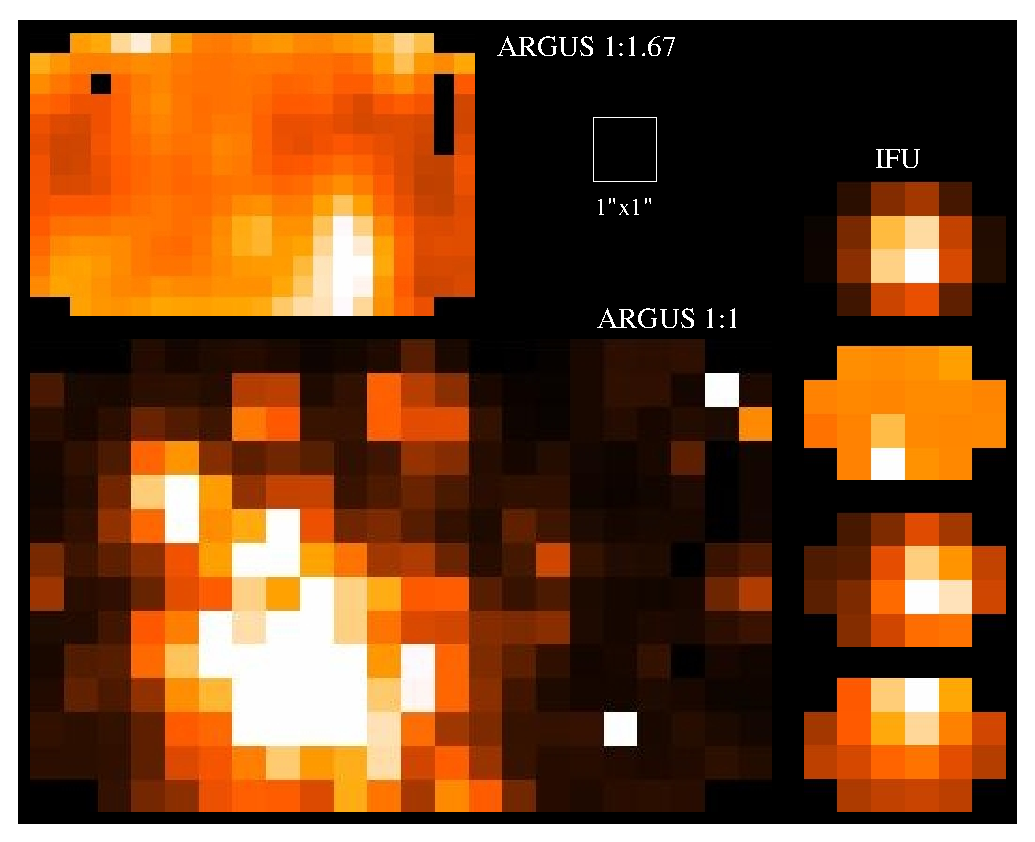
\includegraphics[width=0.6\textwidth]{part6/Royer_P63/P63_f2.eps}
\end{center}
\caption{Sample of spatial thumbnails for 3D data, scaled to the same spatial scale. Are shown four examples of IFU data (4$\times$6 micro-lens arrays covering 2\arcsec$\times$3\arcsec\ on the sky), and two examples of Argus observations (22$\times$14 arrays) one for each spatial scale:  0\farcs 52 (1:1) and 0\farcs 3 per micro-lens (1:1.67). The 1\arcsec$\times$1\arcsec\ spatial scale is also indicated by an open square.}
\label{thumbnails}
\end{figure}

\section{Exploring Both Spatial and Spectral Dimensions}
The\ssindex{Virtual Observatory(VO)} \ssindex{Virtual Observatory (VO)!individual!VO-Paris}VO-Paris Euro3D client is developed by \citet{Chn_08} to deal with 3D spectroscopic datasets. Through interactions using \ssindex{protocols!SAMP}SAMP between \ssindex{applications!Aladin}Aladin\ooindex{Aladin, ascl:1112.019}  and \ssindex{applications!VOSpec}VOSpec\ooindex{VOSpec, ascl:1205.011}, it offers selection and visualization capabilities, spatially and spectrally (Fig\,\ref{aladin}). The input are Euro3D (e.g.  output format of the MMT/Magellan Infrared Spectrograph data reduction \ssindex{data!pipelines!reduction}pipeline) and ``native'' GIRAFFE formats. 
\begin{figure}[!ht]
\begin{center}
    \includegraphics[width=\textwidth]{part6/Royer_P63/P63_f3.eps}
\end{center}
\caption{Screenshots of the interaction between \ssindex{applications!Aladin}Aladin and \ssindex{applications!VOSpec}VOSpec using the\ssindex{Virtual Observatory(VO)} \ssindex{Virtual Observatory (VO)!individual!VO-Paris}VO-Paris Euro3D client \citep{Chn_08} with an observation of the diffuse nebula NGC~6357 in Argus mode. The Argus array if overplotted to an image from the \ssindex{observatories!space-based!HST}HST in \ssindex{applications!Aladin}Aladin (\textbf{a}). The\ssindex{Virtual Observatory(VO)} \ssindex{Virtual Observatory (VO)!individual!VO-Paris}VO-Paris Euro3D client (\textbf{c}) allows a navigation in the array and the display of the corresponding spectrum in \ssindex{applications!VOSpec}VOSpec (\textbf{b}).}
\label{aladin}
\end{figure}


\bibliographystyle{asp2010}

\bibliography{editor}
